\documentclass[letterpaper,11pt]{article}
\usepackage{graphicx}
\usepackage{courier}
\usepackage{amsmath}
\usepackage[left=1.25cm,top=1.5cm,bottom=1.5cm, right=1.65cm,nohead,nofoot]{geometry}
\usepackage{float}
\usepackage{parskip}
\usepackage{url}
\usepackage{multirow}
\usepackage{caption}
\usepackage{outlines}
\usepackage{subfigure}

\newcommand{\dis}{\displaystyle}
\newcommand{\del}{\partial}
\newcommand{\pd}[2]{\frac{\partial #1}{\partial #2}}
\newcommand{\degree}{\circ}
\newcommand{\s}{\text{ }} %one space in math mode
\newcommand{\tab}{\hspace*{0.5 cm}}
\newcommand{\sml}{\tiny}
\newcommand{\med}{\scriptsize}
\newcommand{\norm}{\normalsize}

\author{Daniel Cuneo, Derek Flenniken, Duygu Tosun-Turgut, PhD, Norbert Schuff, PhD}
\title{\begin{center}
\includegraphics[scale = 1.0]{logo.eps}\end{center} \vspace*{4cm} UCSF ASL Perfusion Processing Methods}
\date{\today}

\setlength{\parskip}{0.5cm}
\setlength{\footskip}{1.0cm}

\begin{document}

\begin{titlepage}
\clearpage\maketitle\thispagestyle{empty}
\pagebreak

\tableofcontents
\thispagestyle{empty}
\pagebreak

\end{titlepage}

\section*{Overview}
\addcontentsline{toc}{section}{Overview}
The Center for Imaging of Neurodegenerative Diseases (CIND) processing pipeline for Arterial Spin Label (ASL) imaging, prepares perfusion-weighted images (PWI) and computes a quantitative map of cerebral blood flow (CBF) and a regional analysis. The quantification of CBF and correspondence to high-resolution anatomical MRI data, is achieved by implementing multiple tools from the public domain such as, SPM8 [1], EPI nonlinear geometric distortion correction [2], various FSL tools [3], FreeSurfer [4], Insight Toolkit (ITK) [5] and in house MATLAB scripts. 

In brief, the pipeline performs 1) motion correction of the individual ASL frames, 2) computation of the PWI  by subtracting the mean of tagged  from untagged  ASL data sets, 3) alignment of ASL and structural MRI data, 4) geometric distortion correction, 5) partial volume correction, 6) and CBF quantification in physical units by normalizing ASL to an estimated blood water density signal. 

The outputs include the PWI  and a CBF image, both corrected for EPI distortion in two representations: a) in native perfusion MRI space and b) in the subject-specific space of the corresponding structural MRI data. Each output offers users a variety of options for further processing and analysis of the data, such as subject-specific analysis using anatomical regions of interest or group-specific analysis, such as parametric mapping.In addition, summary measures of CBF within anatomically defined brain regions are provided separately.

\section*{Brief Description of ASL}
\addcontentsline{toc}{section}{Brief Description of ASL}
The concept of ASL provides a means of measuring cerebral blood flow (CBF) completely noninvasive by exploiting the endogenous spins of arterial water as a proxy for blood flow. Labeling (or tagging) is achieved by selectively inverting the magnetization of the arterial spins using MRI principles. After a short delay, allowing the arterial spins to reach the brain, conventional MRI methods are used to map the spatial distribution of the ASL signal. The signal to noise ratio of ASL signal is inherently low due to intense background signal from tissue water. Therefore, the ADNI-2 ASL acquisition protocol requires a set of 52 pairs of repeated tagged and untagged image frames which are then averaged to increase the SNR. 

Many variants of ASL have been developed over the years, such as continuous, pulsed, and velocity selective labeling. Here, we describe a pipeline to process a version of pulsed ASL method  referred to as ``QUIPSS II with thin-slice TI1 periodic saturation" or ``Q2TIPS" [6], augmented by conventional echo-planar imaging (EPI), which has been used in ADNI-2. In Q2TIPS, arterial spins are labeled within a thick $(\approx{10}\s cm)$ inversion slab, placed proximal to the imaging slices, as shown in the figure below. The critical timing parameters of Q2TIPS for quantifying flow are the ASL bolus duration  and the transit delay  from the time of inversion to the time of EPI mapping. 

\begin{figure}[H]
\centering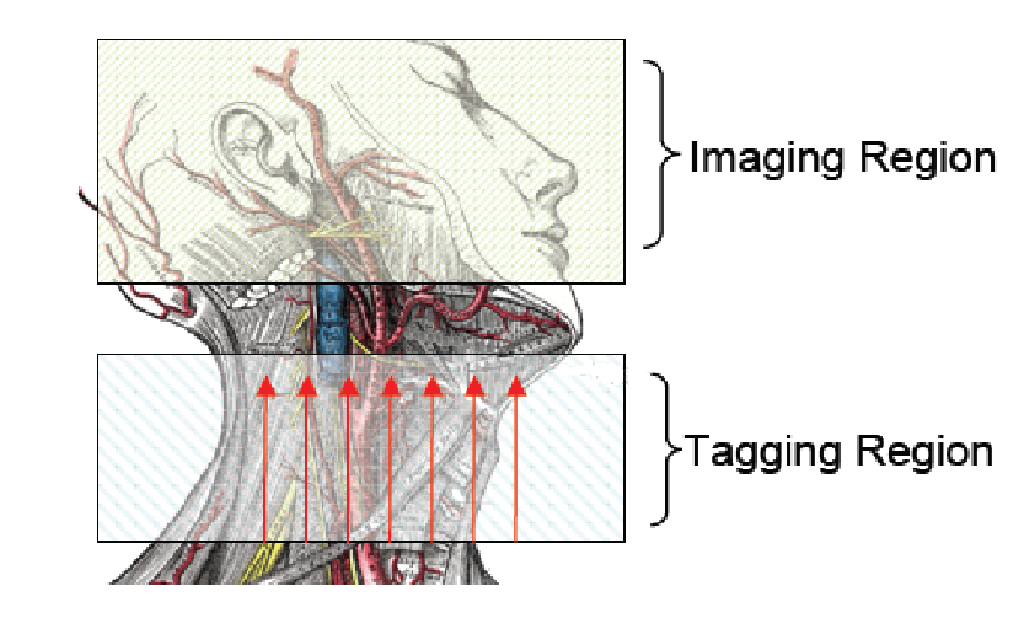
\includegraphics[scale = 0.50]{CBF_regions_diagram.eps}
\caption*{Diagram of ASL regions \newline \med\protect\url{http://www.birncommunity.org/wp-content/uploads/2009/08/4077_Rasmussen.pdf} }
\end{figure}

\section*{ASL-MRI Pre-Processing Steps}
\addcontentsline{toc}{section}{ASL-MRI Pre-Processing Steps}
\begin{enumerate}
\item	Motion Correction: The ASL image series is converted from DICOM to NiFTI format. Each frame is aligned to the first frame to correct for head motion, by a rigid body transformation and least squares fitting, using SPM8.\\

\item	PWI Computations: The ASL images are arranged in groups of tagged and untagged scans and the mean of each group is computed and saved as an image. Then the difference of the mean-tagged and mean-untagged images $(mean_{tagged} - mean_{untagged})$ is taken to obtain a PWI. In addition, the very first untagged ASL image, which provides a fully relaxed MRI signal, is used as a reference of water density and termed $M_{0}$. The reference image is primarily used to calibrate the ASL signal for computations of the CBF and also as an intermediate frame to estimate the transformation to co-register between images from the ASL MRI and structural MRI. In this capacity, the $M_{0}$ is used as the blood-water-density proxy, $M_{blood}$, see below. \\

\item Intensity Scaling: The PWI image as well as the $M_{0}$ image, are intensity scaled. The PWI is scaled  to account for signal decay during acquisition and also to provide intensities in meaningful physical units. The $M_{0}$ is scaled to become  $M_{blood}$, that is, water to blood density.
\end{enumerate}

\emph{{\large \textbf{Description of PWI Scaling}}}:
PWI intensities are corrected for the longitudinal relaxation of the spin tracers during data acquisition, including time lags between consecutive image slices, as well as for incomplete labeling. Assuming an ascending slice order at acquisition with $n=1$ indicating the first slice, the intensity correction for the $n^{th}$ slice is:\\

\begin{align}
\label{eq:scale1}
PWI_{lag-corr} =\dis\frac{PWI_{raw}}{2\alpha{TI_1}}\s e^{\left[R_{1a}(TI_2 + (n - 1)\s\tau )\right]} ,
\end{align} 

where $\alpha$ is the tagging efficiency, $R_{1a}$ is the longitudinal relaxation rate of blood, $TI_1$ is the inversion time of arterial spins and $TI_2$, is the total transit time of the spins, $n$ is the $n^{th}$ slice, and $\tau$ is the time lag between slices.Specific intensity correction parameters used in our implementation are reported in Table 1. R1a is a biological parameter whereas TI1, TI2, and $\tau$ are specific to ADNI-2 acquisition protocol. The resultant image in the native ASL image space is provided in units of blood flow.


\emph{{\large \textbf{Intensity Scaling of $M_0$}}}: 
The control $(M_0)$ image is scaled to estimate a map of the blood magnetization, $M_{blood}$ by correcting for the lower density of tissue water relative to arterial blood water, $\lambda$ , and for the different relaxation characteristics of tissue and arterial blood water,as follows: 

\begin{align}
\label{eq:scale2}
M_{blood} =\dis \frac{M_0}{\lambda} e^{( R^*_{2tissue} -\s R^*_{2blood}) TE} {\text \s ,\s}
\end{align}

where $\lambda$ is the blood/water ratio in tissue, $R^*$ are the two relaxation rates and $TE$ is the blood relaxation time. See table ~\ref{tab:scaleparams} for the parameter values.


\begin{table}[H]
\caption{}
\label{tab:scaleparams}
\centering
\begin{tabular}{|l | l|} \hline
$Parameter$ & Values \\ \hline
$\alpha$  & $0.95$ \\ \hline
$\lambda$ & $0.90$ \\ \hline
$\tau$    & $22.5 \s ms$ \\ \hline
$TE$      & $12$ ms or $13 \s ms$ protocol specific \\ \hline
$TI1$     & $700 \s (ms)$ \\ \hline
$TI2$     & $1900 \s (ms)$ \\ \hline
$R1a$     & $ 1/1684 \s (kHz)$ [8] \\ \hline
$R*_{2tissue}$ & $1/44\s ms$  [9]\\ \hline
$R*_{2blood}$ & $1/43 \s ms$ [10] \\ \hline

\end{tabular}
\end{table} 

\emph{{\large \textbf{Computing A CBF in ASL Space}}}:
A CBF map in the ASL space, can be formed with the $M_{blood}$ and the $PWI_{lag-corr}$, using,
\begin{align}
CBF_{ASL} = \frac{PWI_{lag-corr}}{M_{blood}} \s.
\end{align}


\section*{Structural-to-ASL coregistration and nonlinear  \\ \tab geometric distortion correction}
\addcontentsline{toc}{section}{Structural-to-ASL coregistration and nonlinear  \\ \tab geometric distortion correction}
EPI-based perfusion images suffer from nonlinear geometric distortion due to magnetic susceptibility variations whereas structural MR images are less susceptible to geometric distortions. This is a key challenge in achieving an accurate anatomical match between data from ASL-MRI and structural MRIs. We use a variational image-based approach to correct for these EPI-induced nonlinear geometric distortions in ASL-MRIs.  

The geometric distortion correction step is  performed in the PWI native space. Instead of using the $T2^*$ image, we use a simulated T2 weighted image, made from the $T1$ in the acquisition series. The T2 simulation process is briefly described in the appendix.

The processing steps for nonlinear geometric distortion correction areas follows:
\begin{itemize}
\item $SimT2$  image is masked leaving a layer of sulcal CSF around the brain.
\item $M_{blood}$ is skull stripped with BET [7] and coregistered to the masked T2 using the normalized mutual information metric with 9 degrees of freedom.
\item Masked $SimT2$ is down sampled to the $M_{blood}$ space and named, $T2_{rPWI}$.
\item Distortion correction performed on the $M_{blood}$ using the $T2_{rPWI}$ and the correction field applied to the PWI.
\end{itemize}

\section*{Partial Volume Correction}
\addcontentsline{toc}{section}{Partial Volume Correction}
We are interested in the blood flow of gray matter tissue (GM), which is bounded by cerebrospinal fluid (CSF) and white matter (WM) tissues. To correct for variations in both $PWI_{lag-corr}$ and $M_{blood}$ due to variable coverage of GM, WM and CSF at each voxel, both images are corrected for the tissue partial volume effects before computation of a CBF map. 

Both $PWI_{lag-corr}$ and $M_{blood}$ maps are first upsampled to the T1-weighted MR image space using trilinear interpolation and inverse affine transformation estimated to coregister simulated T2 to masked $M_{blood}$.


The $PWI_{lag-corr}$ intensities are adjusted voxel wise, according to GM and WM tissue density distributions estimated using 4 tissue segmentation provided by SPM8, and assuming a constant ratio between GM and WM matter perfusion. The intensities are corrected according to,

\begin{align}
PWI_{gm} &= \left(PWI_{rT1}\right) \left[\frac{GM}{GM + 0.4 WM} \s.\right]  
\end{align}

Here, $PWI_{rT1}$ is the $PWI_{lag-corr}$ resliced to T1 image space. $\beta{GM}$ and $\beta{WM}$ are the volume fractions of gray matter and white matter respectively.  

In this partial volume model of $PWI_{rT1}$, we assume that signal at each voxel is a weighted linear combination of perfusion from GM and WM, with the weighting coefficients expressing perfusion in terms of the corresponding	tissue	densities (i.e., $\beta_i$ for $i = GM_i \text{ , } WM_i$) and the ratio of GM to WM perfusion is spatially constant at 2.5 value (Kanetaka et al., 2004) [11].

A similar PVC is performed for the $M_{blood}$ . In contrast to PWI, however, partial volume correction for the tissue water reference image needs to include CSF. Partial volume correction of the $M_{blood}$ is computed according to,

\begin{align} 
M_{blood-PVC} = \left( M_{rT1-blood} \right) \left[ \gamma{GM}\left(\gamma^{-1}{GM} + \gamma_1^{-1}{WM} + \gamma_2^{-1}{CSF} \right)\right] + \dis\kappa \s. 
\end{align}

The ratios of tissues to water are, 
$$\gamma = {\frac{GM}{H_2O} = 0.78 \text{ , } \gamma_1 = \frac{WM}{H_2O}= 0.65  \text{ , } \gamma_2 = \frac{CSF}{H_2O}= 0.97}\s,$$  
and
$$\dis\kappa = \frac{1-\sum{(GM+WM+CSF)}}{1\times{10^{100}}}\s.$$

The $\kappa$ parameter is used to regularize the CBF computation (see next section),in the limits where the voxels are entirely made up of gray matter in the CBF ( numerator ) image, or CSF.


\section*{Computation of CBF in T1 Space}
\addcontentsline{toc}{section}{Computation of CBF in T1 Space}
The $PWI_{PVC}$, is normalized by the $M_{blood-PVC}$ to express the ASL signal in physical units of arterial water density$\left(\frac{ml}{100g\s60s}\right)$, yielding CBF according to

\begin{align}
CBF = \frac{PWI_{PVC}}{M_{blood-PVC}} \s.
\end{align}

The $M_{blood}$ in the denominator, is spatially smoothed using a 3D isotropic Gaussian smoothing kernel, whose FWHM is the largest voxel dimension in millimeters, of the native ASL MR image. The normalization also eliminates spatial B1-inhomogeneity by definition, since both maps are subject to the same B1-inhomogeneity distribution. 

The $CBF$ image is also threshold-ed for high intensity outliers by finding the intensity, $C$, that corresponds to $1\%$ of mean CBF signal. The global mean CBF is computed as the center of a the mode in a histogram of the normalized output. CBF intensities are then truncated such that intensities greater than  are set to $C + \epsilon_r$, where $\epsilon_r$ is a random number between zero and one. 

The $CBF$ data type is initially double precision floating point numbers. The final output $CBF$ is saved with a data type of INT32. To preserve the data through this change of data type, the values are scaled up by $1\times{10}^4$. Therefore, all values read from a viewer must be divided by $1 \times 10^4$ to obtain CBF in units of $ml/100mg/min$ .

\begin{align}
\label{eq:outputScale}
CBF = \frac{voxel \s intensity}{1\times{10}^4}
\end{align}

\section*{Free Surfer ROI Statistics}
\addcontentsline{toc}{section}{Free Surfer ROI Statistics}
In addition to the CBF image, ROI statistics from anatomical regions of interest are also computed, from the CBF image in T1 space. FreeSurfer is used to segment sub-cortical structures and parcellate the cortical surface into regions of interest (ROI). Because the ASL-MRI acquisition might have partial brain coverage (e.g., possible temporal and occipital cut-offs), FreeSurfer ROIs are truncated with a non-zero CBF brain mask. An Insight\-Toolkit (ITK) based in house C++ program is then employed to compute the quantities listed below. The output is a space delimited text file named `ROIperfusion.log' and contains only regions with a non-zero count of voxels in the ROI.

\begin{table}[H]
\begin{itemize} 
\item number of voxels in the ROI
\item minimum  
\item maximum  
\item mean     
\item median   
\item standard deviation 
\end{itemize}
\end{table}

\section*{CBF Output Quality Control (QC) Criteria and Steps}
\addcontentsline{toc}{section}{CBF Output Quality Control (QC) Criteria and Steps}
\begin{outline}[enumerate]
\1	Image Quality QC
\2  Raw Data QC: Pass/Fail
\3	This is the only level where we are making a judgment based on the image quality.
\3	All data is run regardless of QC

\1	Processing QC: Registration check to determine the success of the processing pypeline
\2	Registration QC: The output image check and the only category that determines exclusion from uploads. 
\3	This QC is performed by overlaying the Final\_Mblood file (``SubjectCode\_Mblood-EpiCorr-rT1-PVC-Smoothed.nii'') onto the raw T1            (``SubjectCode \_T1.nii'').  
\3	Pass: Mblood overlays completely onto T1.  Verified by checking brain edges and, if possible, Vents.
\3	Follow-up:  Anything strange; brain edges not aligned, Ventricles off, or perhaps a 3D lateral shift
\3  Note: We are not doing a QC on the quality of the MBlood image.  So any signal loss in the extremities like inferior temps or           medialorbitofrontal does not affect the rating.  We are checking for a successful registration only.
\2	There is no rating of Fail in the processing QCs because at the moment we are attempting to resolve all issues that require             follow-up.
\end{outline}

\vspace*{1cm}

\begin{figure}[H]
\centering
\caption*{Mblood-EpiCorr-rT1-PVC-Smoothed.nii}
\mbox{\subfigure{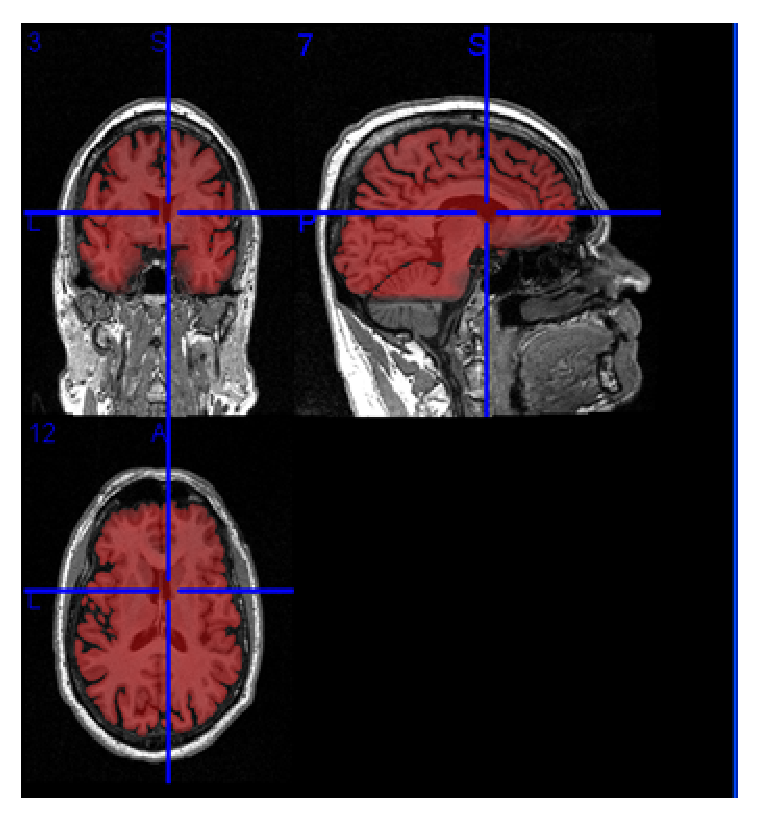
\includegraphics[scale = 0.45]{qc-pass.eps}}}\quad
\subfigure{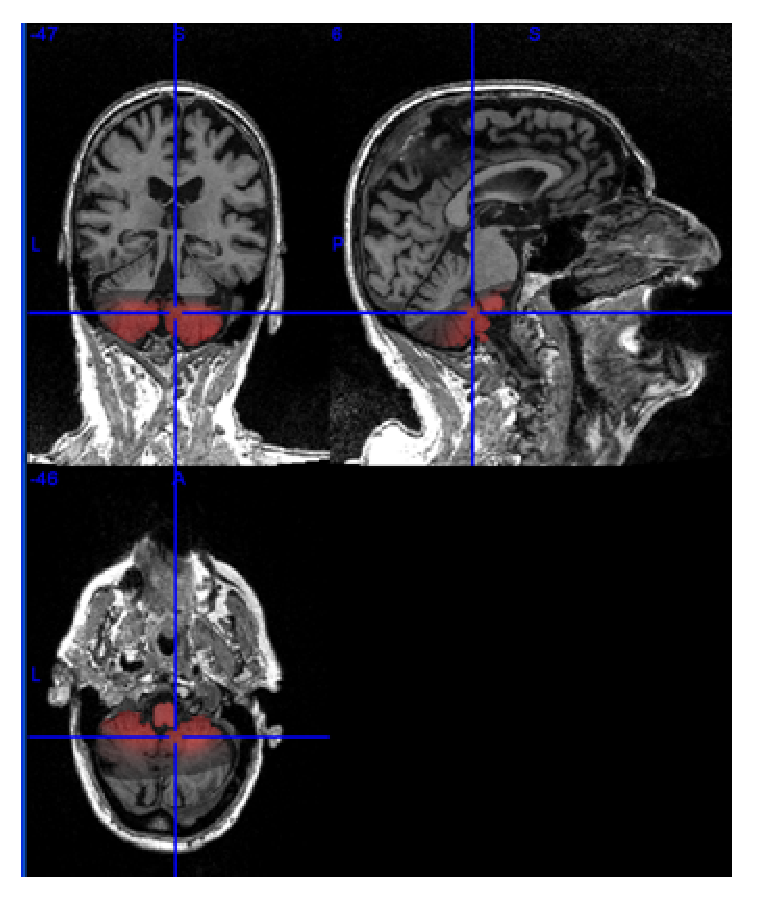
\includegraphics[scale = 0.42]{qc-fail.eps}}
\caption*{QC Registration \emph{Pass} \hspace*{2.5cm} QC Registration \emph{Follow Up}}
\end{figure}

\section*{Limitations}
\addcontentsline{toc}{section}{Limitations}
\begin{enumerate}
\item \emph{DEFORMATION FIELD}: The method of variational matching for the distortion correction in ASL does not account for intensity variations due to pixel aliasing. Thus, ASL values from regions with prominent susceptibility distortions should be interpreted with caution.\\

\item \emph{INTENSITY SCALING}: The current implementation of intensity scaling of PWI and $M_{0}$ maps does not account for regional and subject-specific variations in the signal relaxation rates. Moreover, the scaling of PWI does not account for regional and subject-specific variations in transit delays of the ASL bolus. Therefore, a bias in scaling is introduced to the extent that signal relaxation rates and transit delays vary across regions and subjects. \\

\item	\emph{PARTIAL VOLUME CORRECTION}: The current implementation of partial volume correction does not account for regional variations in the ratio of gray matter to white matter perfusion nor is the ratio value driven by the data. Therefore, a bias in gray matter perfusion is introduced to the extent that the ratio varies across regions and subjects. 
\end{enumerate}


%%%%%%%%%%%%%%%%%%%% OUTPUT SUMMARY %%%%%%%%%%%%%%%%%%%%%%%%%%%%
{\centering

\begin{table}[H]
\begin{tabular}{l @{  ................................................  }l }
\multicolumn{2}{c}{\textbf{{\norm OUTPUT SUMMARY}}} \\[1.5ex]

\multicolumn{2}{l}{\textbf{EPI Corrected ASL Space}} \\[1.5ex]      

\begin{med}\emph{Theoretical Name}\end{med} & \begin{med}\emph{Filename}\end{med} \\[1.5ex]

$PWI_{scaled-epi-corr}$ & {\ttfamily ScaledPWI-aACPC-EpiCorr.nii} \\
$M_{blood-EpiCorr}$    & {\ttfamily Mblood-EpiCorr.nii}    \\[1.5ex]                

\multicolumn{2}{l}{\textbf{T1 Space}} \\[1.5ex] 

$PWI_{scaled-EpiCorr-rT1}$ & {\ttfamily ScaledPWI-aACPC-EpiCorr-rT1.nii} \\
$M_{blood-EpiCorr-rT1}$ & {\ttfamily Mblood-EpiCorr-rT1.nii}        \\[1.5ex]

GM  segmentation image & {\ttfamily T1-GmMask.nii} \\
WM  segmentation image & {\ttfamily T1-WmMask.nii} \\
CSF segmentation image & {\ttfamily T1-CsfMask.nii} \\[1.5ex]


$PWI_{scaled-EpiCorr-rT1-pvc}$ & {\ttfamily ScaledPWI-aACPC-EpiCorr-rT1-PVC.nii} \\
$M_{blood-EpiCorr-rT1-pvc}$    & {\ttfamily Mblood-EpiCorr-rT1-PVC.nii}  \\[1.5ex]  

$CBF$ & {\ttfamily ScaledPWI-aACPC-EpiCorr-rT1-PVC-Norm.nii} \\[1.5ex]

\multicolumn{2}{l}{\textbf{FreeSurfer ROI Statistics}} \\[1.5ex]
First order statistics per  ROI  & {\ttfamily ROIperfusion.log}

\end{tabular}
\end{table}
} % end centering


\pagebreak
\section*{Processing Steps Flow Diagram}
\addcontentsline{toc}{section}{Processing Steps Flow Diagram}
\begin{figure}[H]
\centering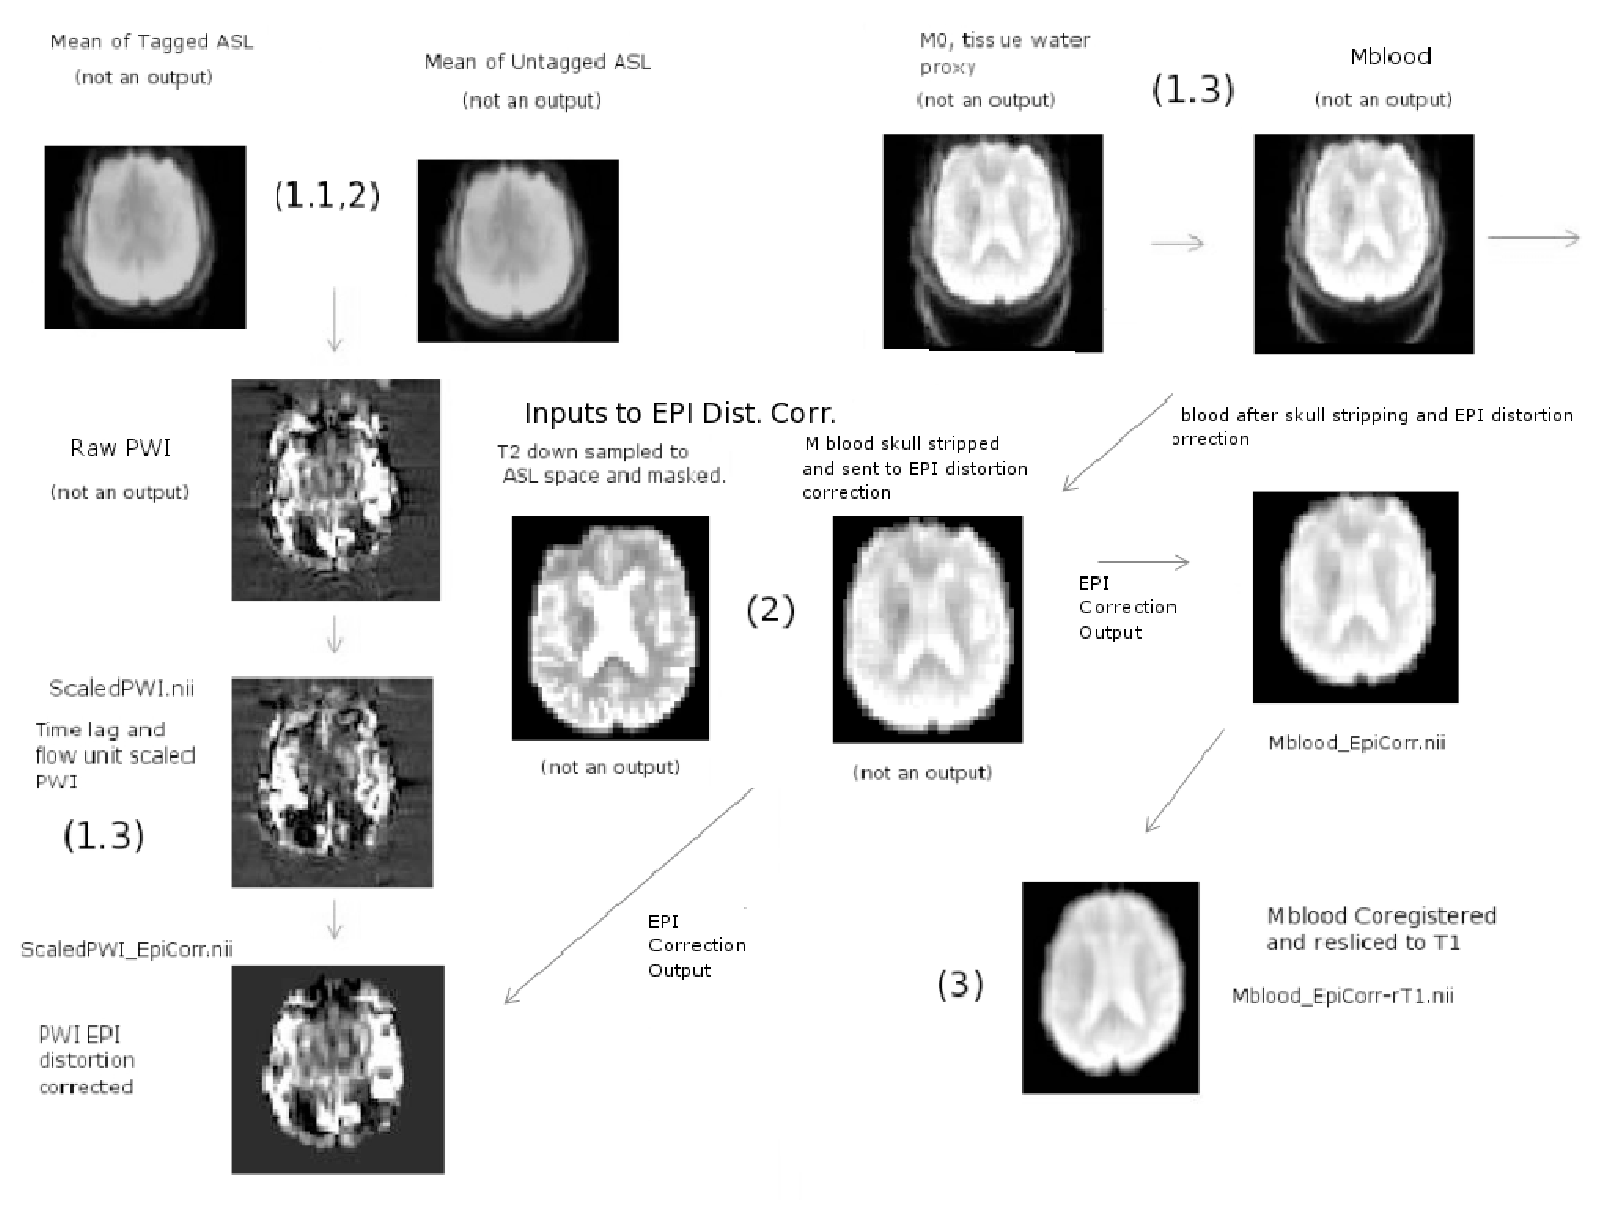
\includegraphics[scale = 0.70]{flow_diagram_revised_1.eps}
\centering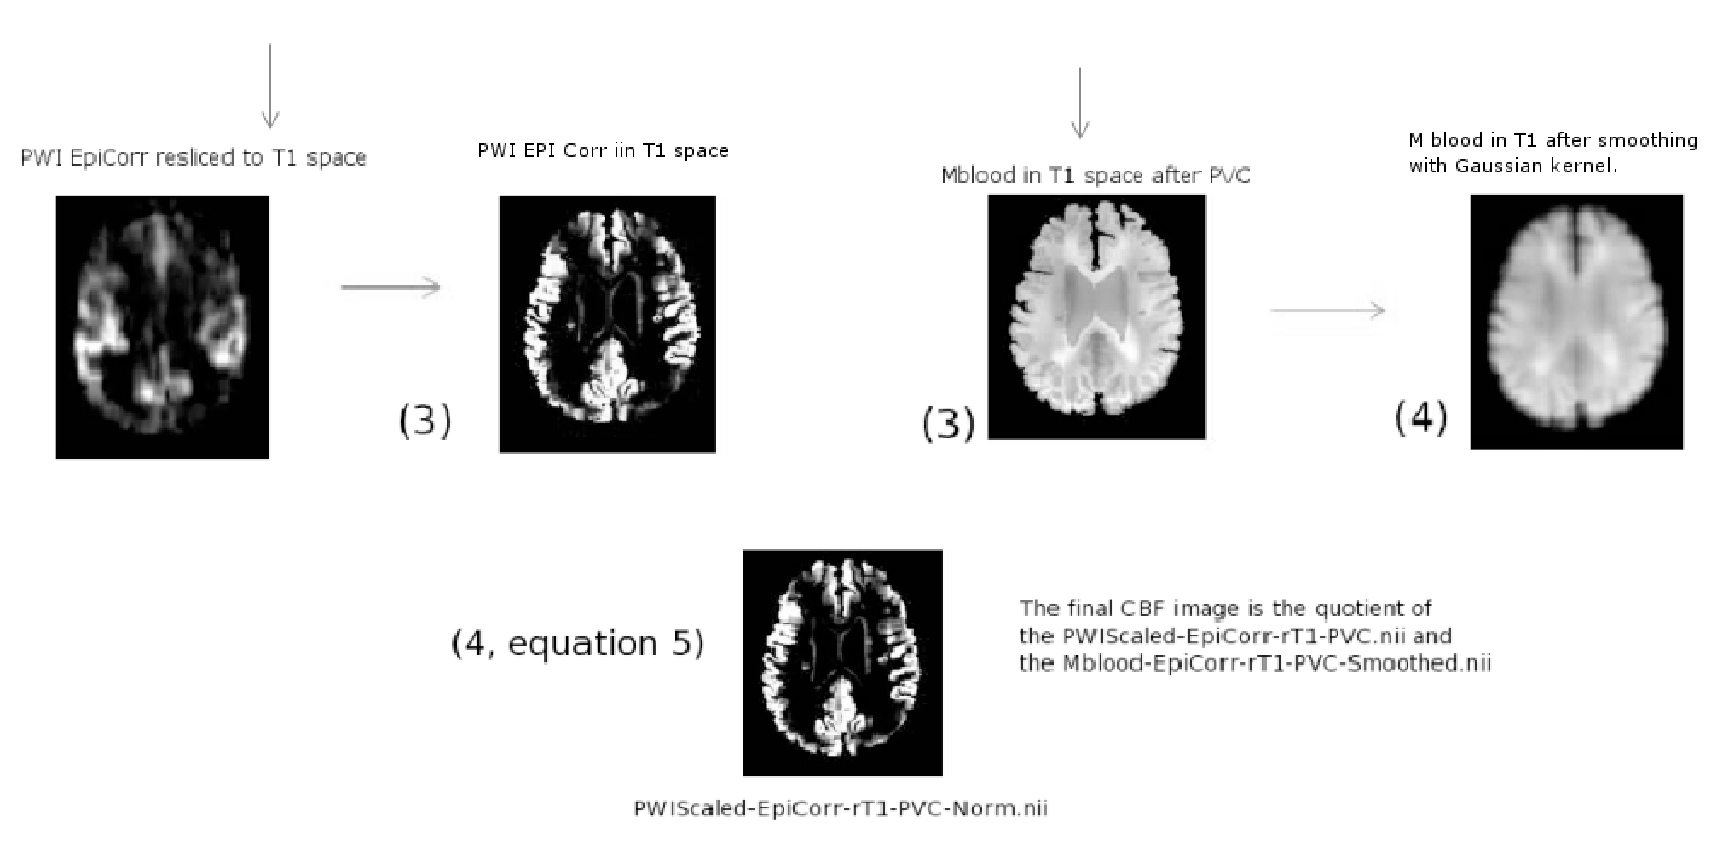
\includegraphics[scale = 0.65]{flow_diagram_revised_2.eps}
\end{figure}

\section*{Appendix: Simulated T2-weighted MRI}
\addcontentsline{toc}{section}{Simulated T2-weighted MRI}
A framework to simulate subject-specific T2-weighted MR images was engineered by Dr Duygu Tosun-Turgut. The framework is based on the work by Benoit-Cattin et al.[12] To mimic clinical neuroimaging practice, we chose the following 2D Turbo Spin Echo (TSE) sequence parameters for simulated T2-MRI. 

{\centering
\begin{table}[H]
\centering
\begin{tabular}{|l|r|} \hline 
Parameter & Value     \\ \hline \hline
TR & $3210 \s ms$     \\ \hline
TE & $101 \s ms$      \\ \hline
slice thickness & $3\s mm$   \\ \hline
resolution & $1\times{1}\s mm$  \\ \hline
flip angle & $150^{\circ}$        \\ \hline
bandwidth & 185\s Hz         \\ \hline
GRAPPA  & $2$              \\ \hline
\end{tabular}
\end{table}
}

T2-MRI simulation steps are as follows:

In brief, the steps to make a simulated T2 are:
\begin{itemize}
\item	Create a binary brain tissue mask from FreeSurfer 'aparc+aseg' anatomical annotation.
\item	Apply a morphological closing operator followed by a morphological dilation to eliminate holes in brain mask and to include sulcal CSF.
\item	Apply resulting brain mask to T1-MRI, yielding skull-stripped T1 image.
\item	Downsample skull-stripped T1 image to $1\times{1}\times{3} \s mm^{3}$ image resolution to mimic clinical neuro imaging practice.
\item	Apply a fuzzy c-means clustering algorithm to estimate GM,WM, and CSF tissue density at each image voxel in downsampled skull-stripped T1 image space
\item	Based on selected acquisition parameters and tissue density estimates, simulate a T2-MRI.
\end{itemize}
Each 2D axial slice is simulated separately and finally merged back to form a simulated 3D T2-MRI.

\section*{Data Set Information}
\addcontentsline{toc}{section}{Data Set Information}

\begin{tabular}{c c}
UCSF ASL FS & Uploaded on November 1st, 2012 \\ 
\end{tabular}

\section*{References}
\addcontentsline{toc}{section}{References}
\begin{enumerate}
\item  \url{http://www.fil.ion.ucl.ac.uk/spm/} \\
\item  Ran Tao, P. Thomas Fletcher, et al. (2009). "A Variational Image-Based Approach to the Correction of Susceptibility Artifacts in the Alignment of Diffusion Weighted and Structural MRI." Process Med Imaging 21: 664-675.  \\
\item \url{http://www.fmrib.ox.ac.uk/fsl/} \\
\item  \url{http://surfer.nmr.mgh.harvard.edu/fswiki/FreeSurferMethodsCitation} \\
\item T.S. Yoo, M. J. Ackerman, W. E. Lorensen, W. Schroeder, V. Chalana, S. Aylward, D. Metaxes, R. Whitaker. Engineering and Algorithm Design for an Image Processing API: A Technical Report on ITK - The Insight Toolkit. In Proc. of Medicine Meets Virtual Reality, J. Westwood, ed., IOS Press Amsterdam pp 586-592 (2002). 
\item  Luh et al., Magn. Reson. Med. 41:1246-1254 (1999) \\
\item S.M. Smith, Fast robust automated brain extraction; Human Brain Mapping,
17(3):143-155, November 2002.
\item Lu at al., Magn. Reson. Med. 52(3):679-82;(2004) \\
\item Donahue et al., Magn. Reson. Med. 56:1261-73;(2006) \\
\item Zhao et al.Magn. Reson. Med. 58:592-97;(2007)
\item Kanetaka, H., Matsuda, H., Asada, T., Ohnishi, T., Yamashita, F., Imabayashi, E., Tanaka, F., Nakano, S., Takasaki, M., 2004. Effects of partial volume correction on discrimination between very early Alzheimer's dementia and controls using brain perfusion SPECT. Eur. J. Nucl. Med. Mol. Imaging 31, 975-980.
\item H. Benoit-Cattin, G. Collewet, B. Belaroussi, H. Saint-Jalmes, C. Odet, The SIMRI project: a versatile and interactive MRI simulator, Journal of Magnetic Resonance, Volume 173, Issue 1, March 2005, Pages 97-115, ISSN 1090-7807, 10.1016/j.jmr.2004.09.027.


\end{enumerate}

\section*{Contact Information}
\addcontentsline{toc}{section}{Contact Information}
This document was prepared by Daniel Cuneo, UCSF/SF VA Medical Center. For more information please contact Alix Simonson at \url{alix.simonson@va.gov} or Diana Truran-Sacrey at \url{diana.truran@ucsf.edu}.

\end{document}
